% !TEX encoding = UTF-8 Unicode
%!TEX root = ../Main/thesis.tex
% !TEX spellcheck = en-US
%%=========================================
\documentclass[../Main/thesis.tex]{subfiles}
\begin{document}
\chapter{Visualizations from the final evaluation}
\label{app:visualizations}

\begin{figure}[h]
	\centering
	\begin{subfigure}{0.45\textwidth}
		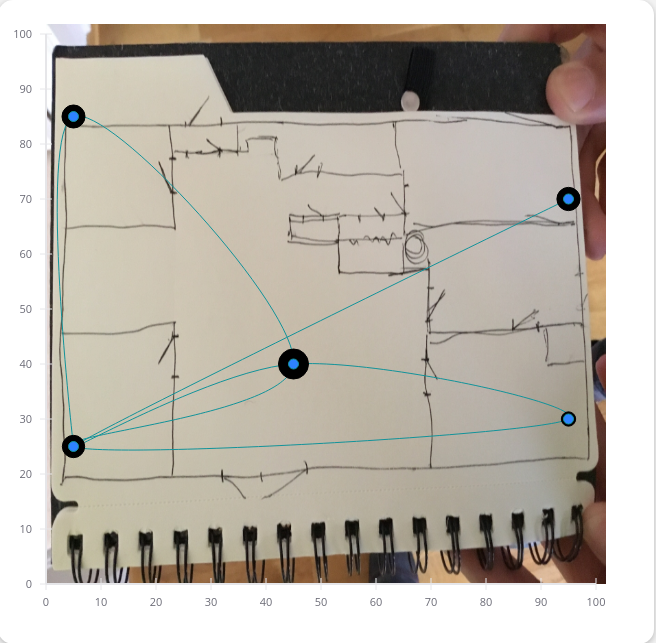
\includegraphics[width=\textwidth]{../fig/eval_1_remi}
		\caption{Smoke diver 1}
		\label{fig:eval-visualization-1-1-app}
	\end{subfigure}
	\caption{Visualization from exercise 1}
	\label{fig:eval-visualization-1-app}
\end{figure}

\begin{figure}[h]
	\centering
	\begin{subfigure}{0.45\textwidth}
		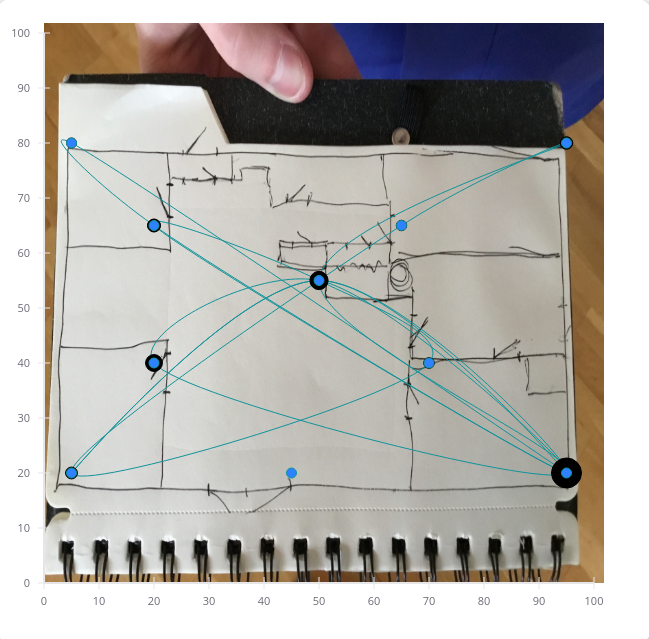
\includegraphics[width=\textwidth]{../fig/eval_2_remi}
		\caption{Smoke diver 1}
		\label{fig:eval-visualization-2-1-app}
	\end{subfigure}
	\begin{subfigure}{0.45\textwidth}
		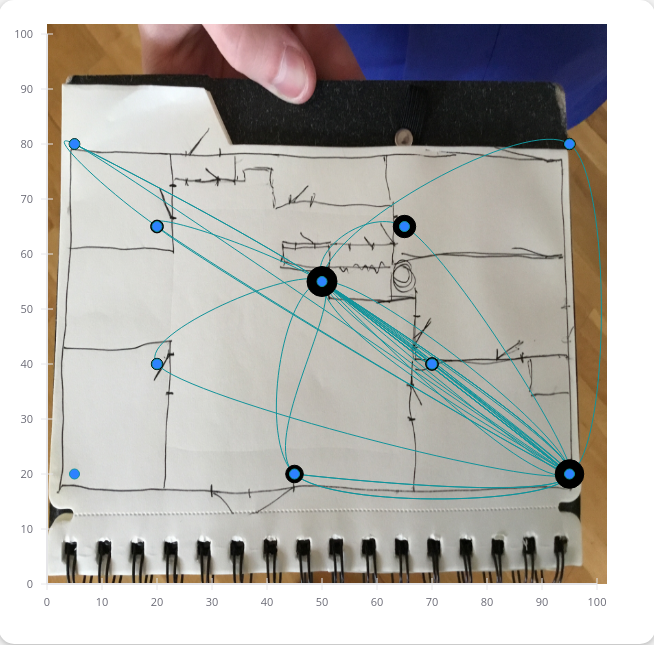
\includegraphics[width=\textwidth]{../fig/eval_2_fredrik}
		\caption{Smoke diver 1}
		\label{fig:eval-visualization-2-2-app}
	\end{subfigure}
	\caption{Visualizations from exercise 2}
	\label{fig:eval-visualization-2-app}
\end{figure}

\begin{figure}[h]
	\centering
	\begin{subfigure}{0.45\textwidth}
		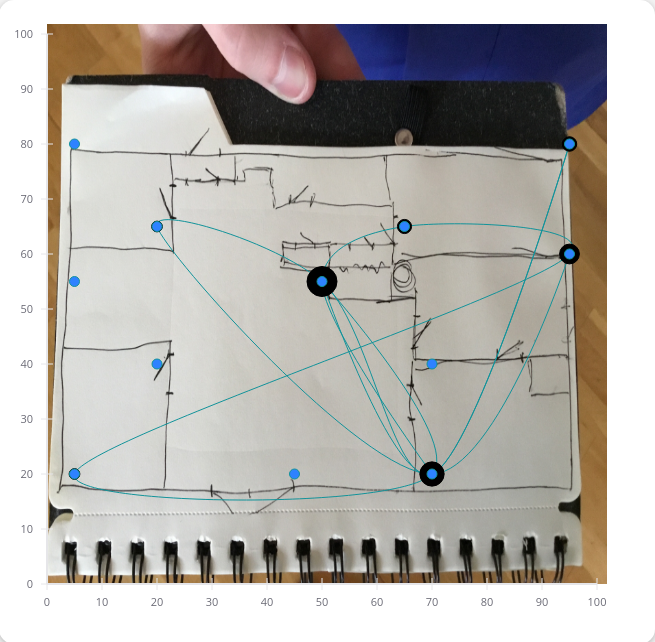
\includegraphics[width=\textwidth]{../fig/eval_3_remi}
		\caption{Smoke diver 2}
		\label{fig:eval-visualization-3-1-app}
	\end{subfigure}
	\begin{subfigure}{0.45\textwidth}
		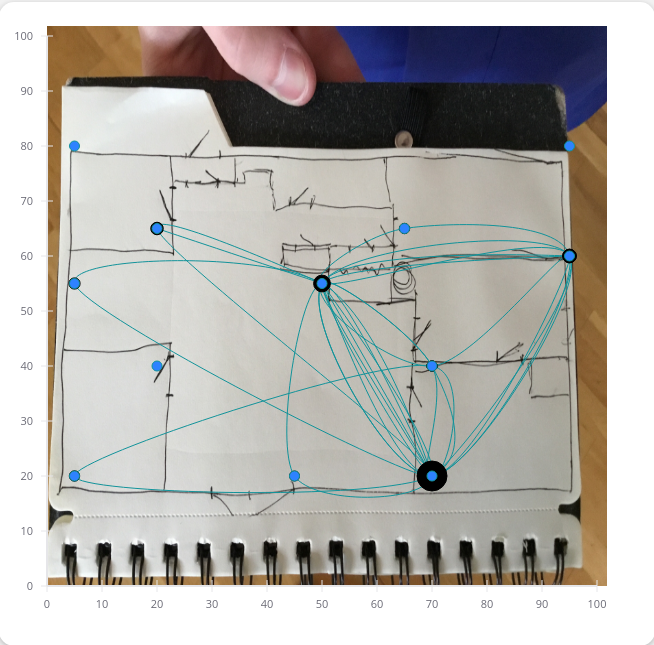
\includegraphics[width=\textwidth]{../fig/eval_3_fredrik}
		\caption{Smoke diver 1}
		\label{fig:eval-visualization-3-2-app}
	\end{subfigure}
	\caption{Visualizations from exercise 3}
	\label{fig:eval-visualization-3-app}
\end{figure}

\begin{figure}[h]
	\centering
	\begin{subfigure}{0.45\textwidth}
		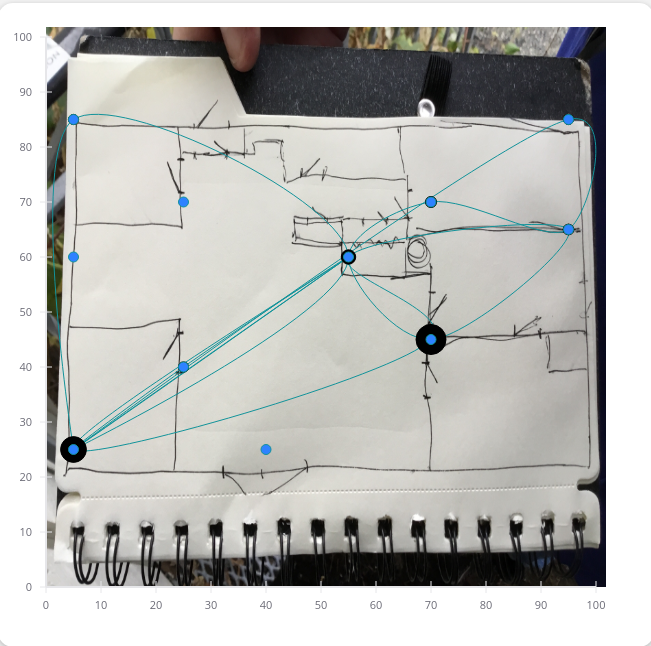
\includegraphics[width=\textwidth]{../fig/eval_4_1}
		\caption{Smoke diver}
		\label{fig:eval-visualization-4-1-app}
	\end{subfigure}
	\begin{subfigure}{0.45\textwidth}
		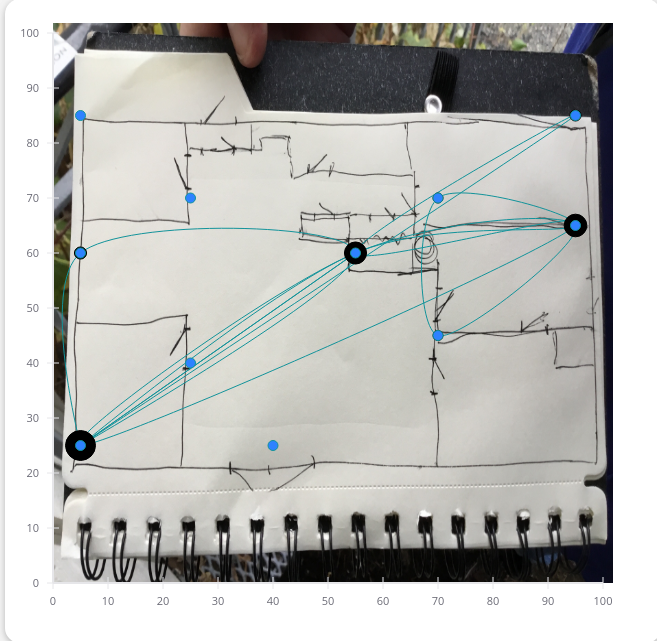
\includegraphics[width=\textwidth]{../fig/eval_4_2}
		\caption{Instructor}
		\label{fig:eval-visualization-4-2-app}
	\end{subfigure}
	\caption{Visualizations from exercise 4}
	\label{fig:eval-visualization-4-app}
\end{figure}

\end{document}
